%%%%%%%%%%%%%%%%%%%%%%%%%%%%%%%%%%%%%%%%%
% Fancyslides Presentation
% LaTeX Template
% Version 1.0 (30/6/13)
%
% This template has been downloaded from:
% http://www.LaTeXTemplates.com
%
% The Fancyslides class was created by:
% Paweł Łupkowski (pawel.lupkowski@gmail.com)
%
% License:
% CC BY-NC-SA 3.0 (http://creativecommons.org/licenses/by-nc-sa/3.0/)
%
%%%%%%%%%%%%%%%%%%%%%%%%%%%%%%%%%%%%%%%%%

%----------------------------------------------------------------------------------------
%	PACKAGES AND OTHER DOCUMENT CONFIGURATIONS
%----------------------------------------------------------------------------------------

\documentclass{fancyslides}

\usepackage[utf8]{inputenc} % Allows the usage of non-english characters
\usepackage{times} % Use the Times font
\usepackage{booktabs} % Allows the use of \toprule, \midrule and \bottomrule in tables
\graphicspath{{images/}} % Location of the slide background and figure files

% Beamer options - do not change
\usetheme{default} 
\setbeamertemplate{navigation symbols}{} % Disable the slide navigation buttons on the bottom of each slide
\setbeamercolor{structure}{fg=\yourowntexcol} % Define the color of titles and fixed text elements (e.g. bullet points)
\setbeamercolor{normal text}{fg=\yourowntexcol} % Define the color of text in the presentation

%------------------------------------------------
% COLORS
% The following colors are predefined in this class: white, black, gray, blue, green and orange

% Define your own color as follows:
%\definecolor{pink}{rgb}{156,0,151}

\newcommand{\structureopacity}{0.75} % Opacity (transparency) for the structure elements (boxes and circles)

\newcommand{\strcolor}{blue} % Set the color of structure elements (boxes and circles)
\newcommand{\yourowntexcol}{white} % Set the text color

%----------------------------------------------------------------------------------------
%	TITLE SLIDE
%----------------------------------------------------------------------------------------

\newcommand{\titlephrase}{Sportangebot der HTW
} % Presentation title
\newcommand{\name}{Gilles Baatz, Jan Jochum, Tobias Kalmes, Frantz Tenguemne, Michael Wolf
} % Presenter's name
\newcommand{\affil}{HTW des Saarlandes} % Presenter's institution
\newcommand{\email}{Semantische Interoperabilität} % Presenter's email address

\begin{document}

\startingslide % This command inserts the title slide as the first slide

%----------------------------------------------------------------------------------------
%	PRESENTATION SLIDES
%----------------------------------------------------------------------------------------

\fbckg{hurdles_1b.jpg} % Slide background image
\begin{frame}
\pointedsl{Ziel} % Text in this environment is printed in a circle and will be made large and uppercase - if you need to fit more text in you can reduce the font size within the \pointedsl{} bracket as usual, e.g. \pointedsl{\large smaller main point}
\end{frame}

%------------------------------------------------

%\fbckg{2.jpg} % Slide background image
%\begin{frame}
%\framedsl{explained clearly with more text} % Text in this environment will be made large, uppercase and will wrap multiple lines
%\end{frame}

%------------------------------------------------

\fbckg{hurdles_1b.jpg} % Slide background image
\begin{frame}
\itemized{ % This environment simply prints a series of bullet points
\item Hochschulsportberater
\item Schwerpunkt Ontologie
}
\end{frame}

%------------------------------------------------

\fbckg{onto_1b.jpg} % Slide background image
\begin{frame}
\pointedsl{Ontologie} % Text in this environment is printed in a circle and will be made large and uppercase - if you need to fit more text in you can reduce the font size within the \pointedsl{} bracket as usual, e.g. \pointedsl{\large smaller main point}
\end{frame}

%------------------------------------------------

\fbckg{onto_1b.jpg} % Slide background image
\begin{frame}
\framedsl{Wissen des Beraters} % Text in this environment will be made large, uppercase and will wrap multiple lines
\end{frame}

%------------------------------------------------

\fbckg{people_1.jpg} % Slide background image
\begin{frame}
\framedsl{Personenarten} % Text in this environment will be made large, uppercase and will wrap multiple lines
\end{frame}

%------------------------------------------------

\fbckg{source_1.jpg} % Slide background image
\begin{frame}
\pointedsl{Vorführung} % Text in this environment will be made large, uppercase and will wrap multiple lines
\end{frame}

%------------------------------------------------

\fbckg{blank} % A blank background can be used instead of an image
\begin{frame}
\sources{ % An environment for giving credit for slide backgrounds, images will need to be scaled down if there are more than two
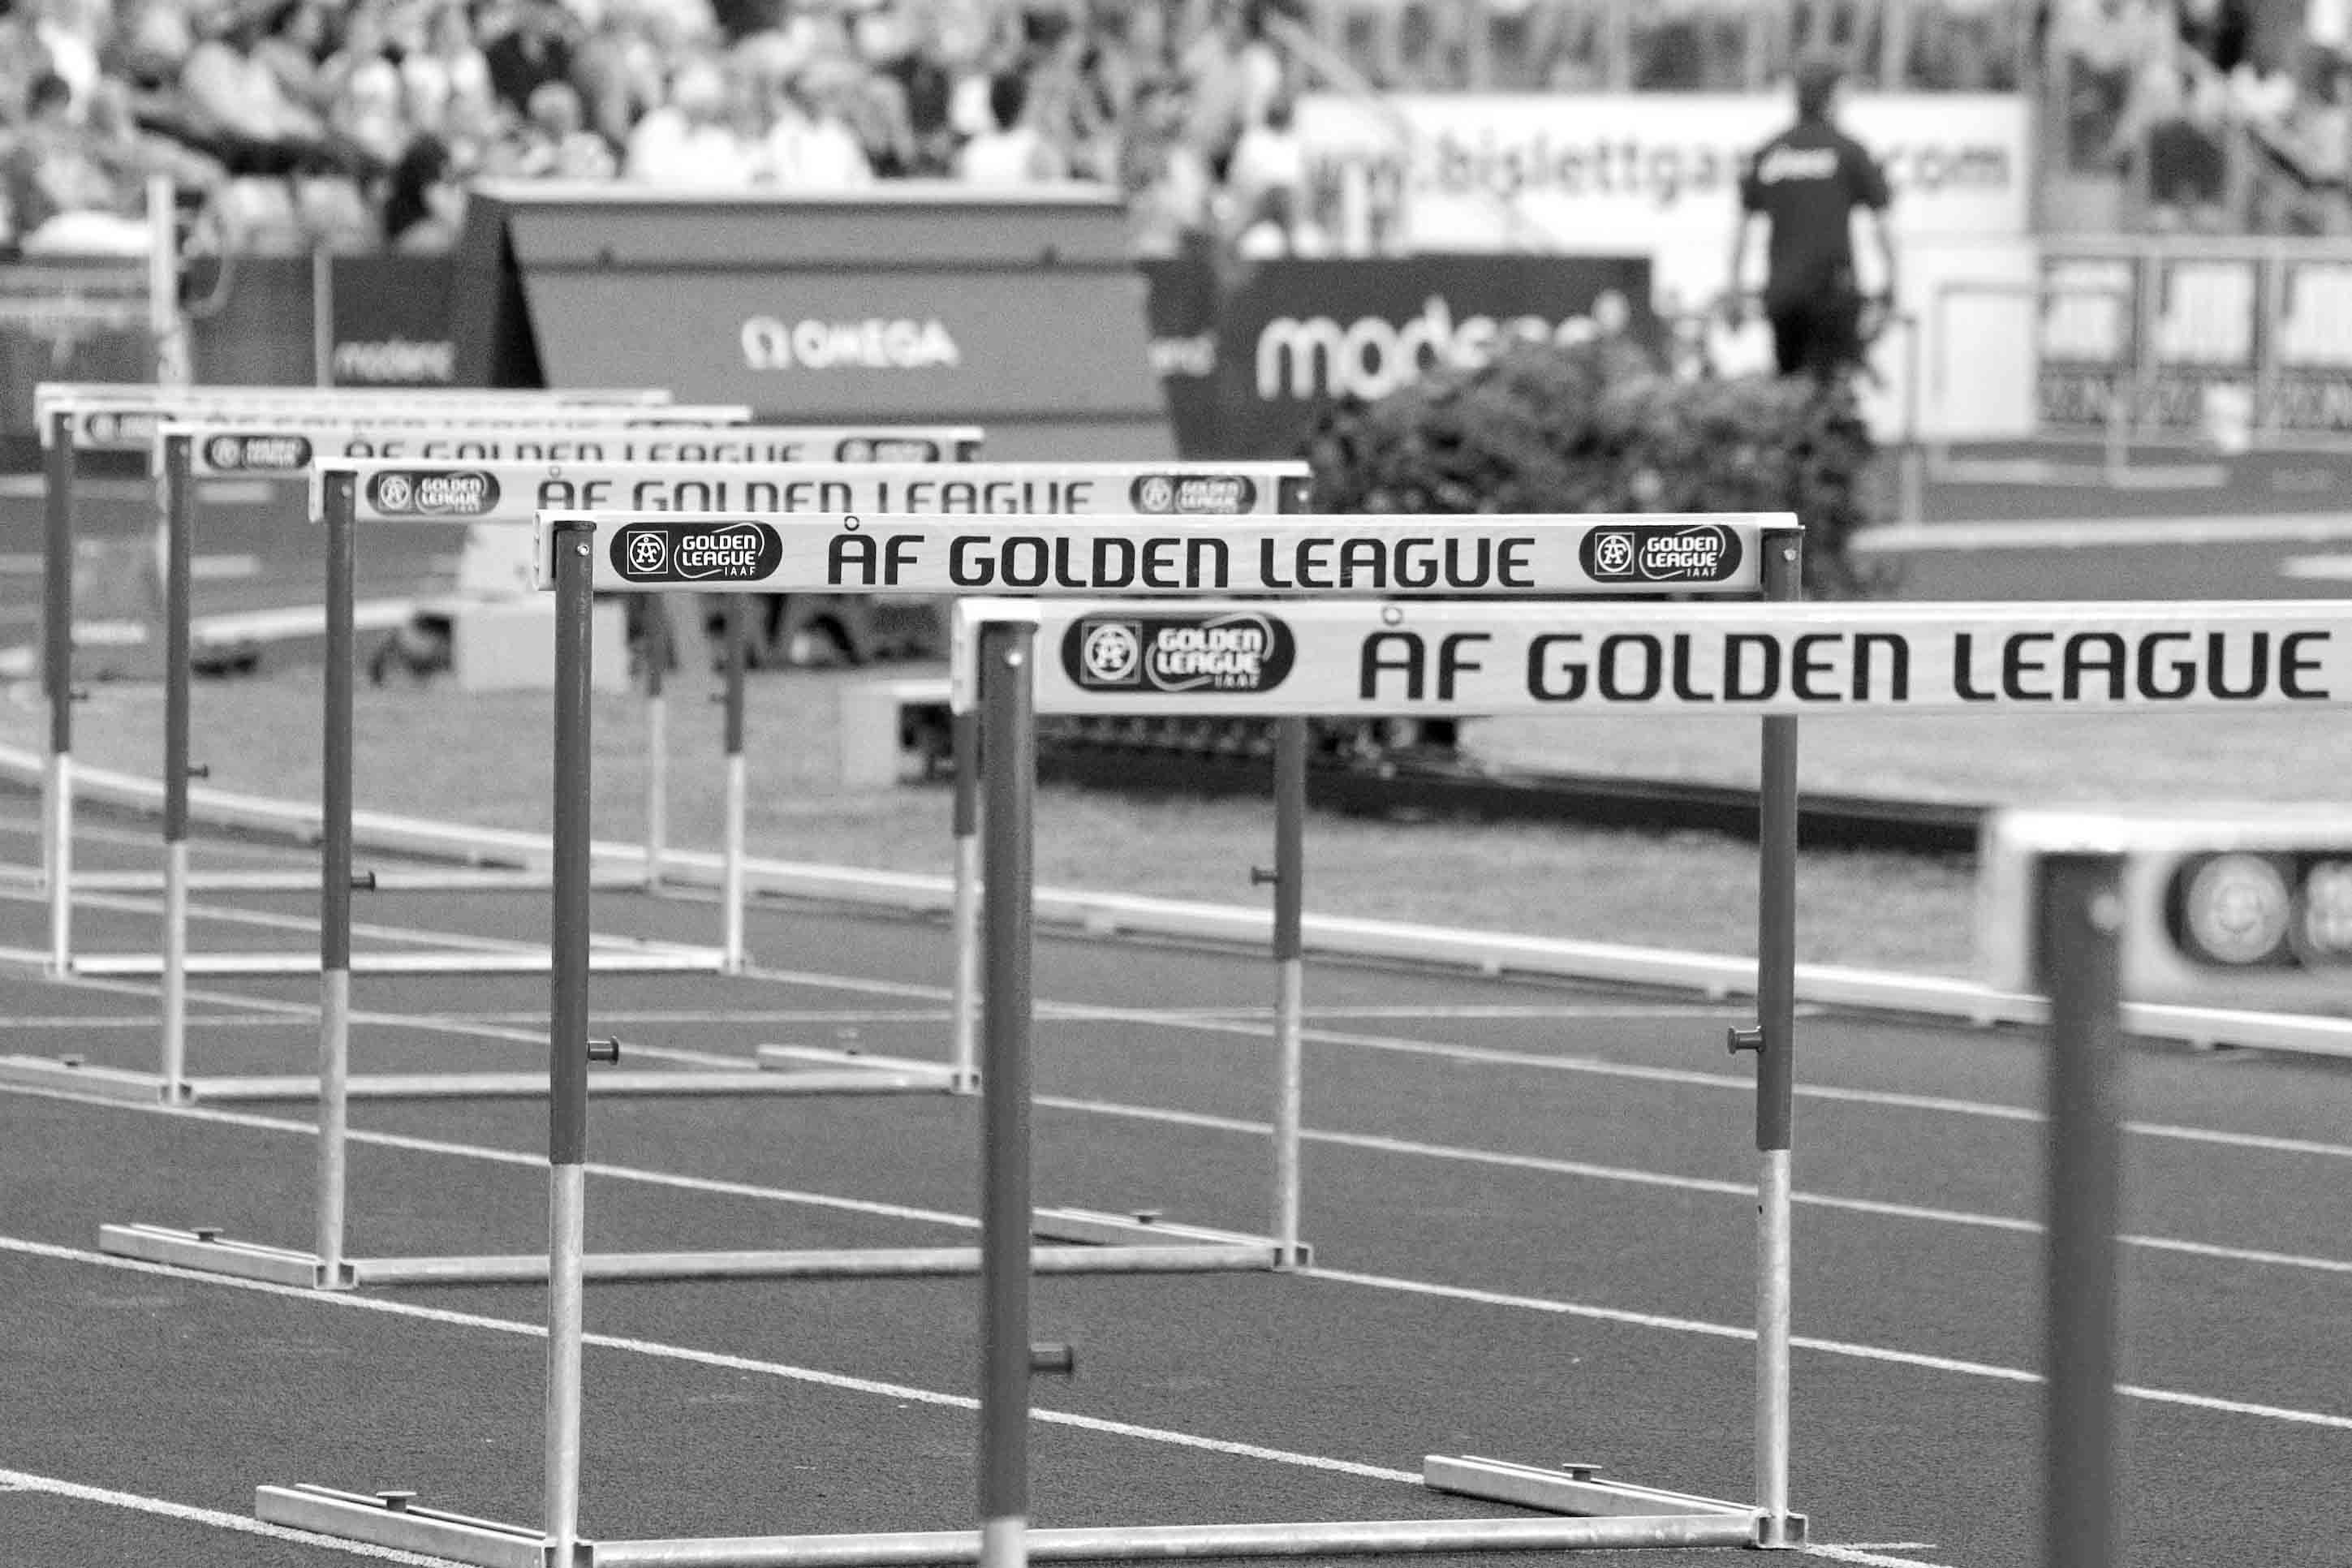
\includegraphics[width=0.25\paperwidth]{hurdles_1b}Ragnar Singsaas, Exxon Mobil ÅF Golden League Bislett Games 2008, 07.07.2008 via Flickr, Creative Commons Attribution-ShareAlike\\
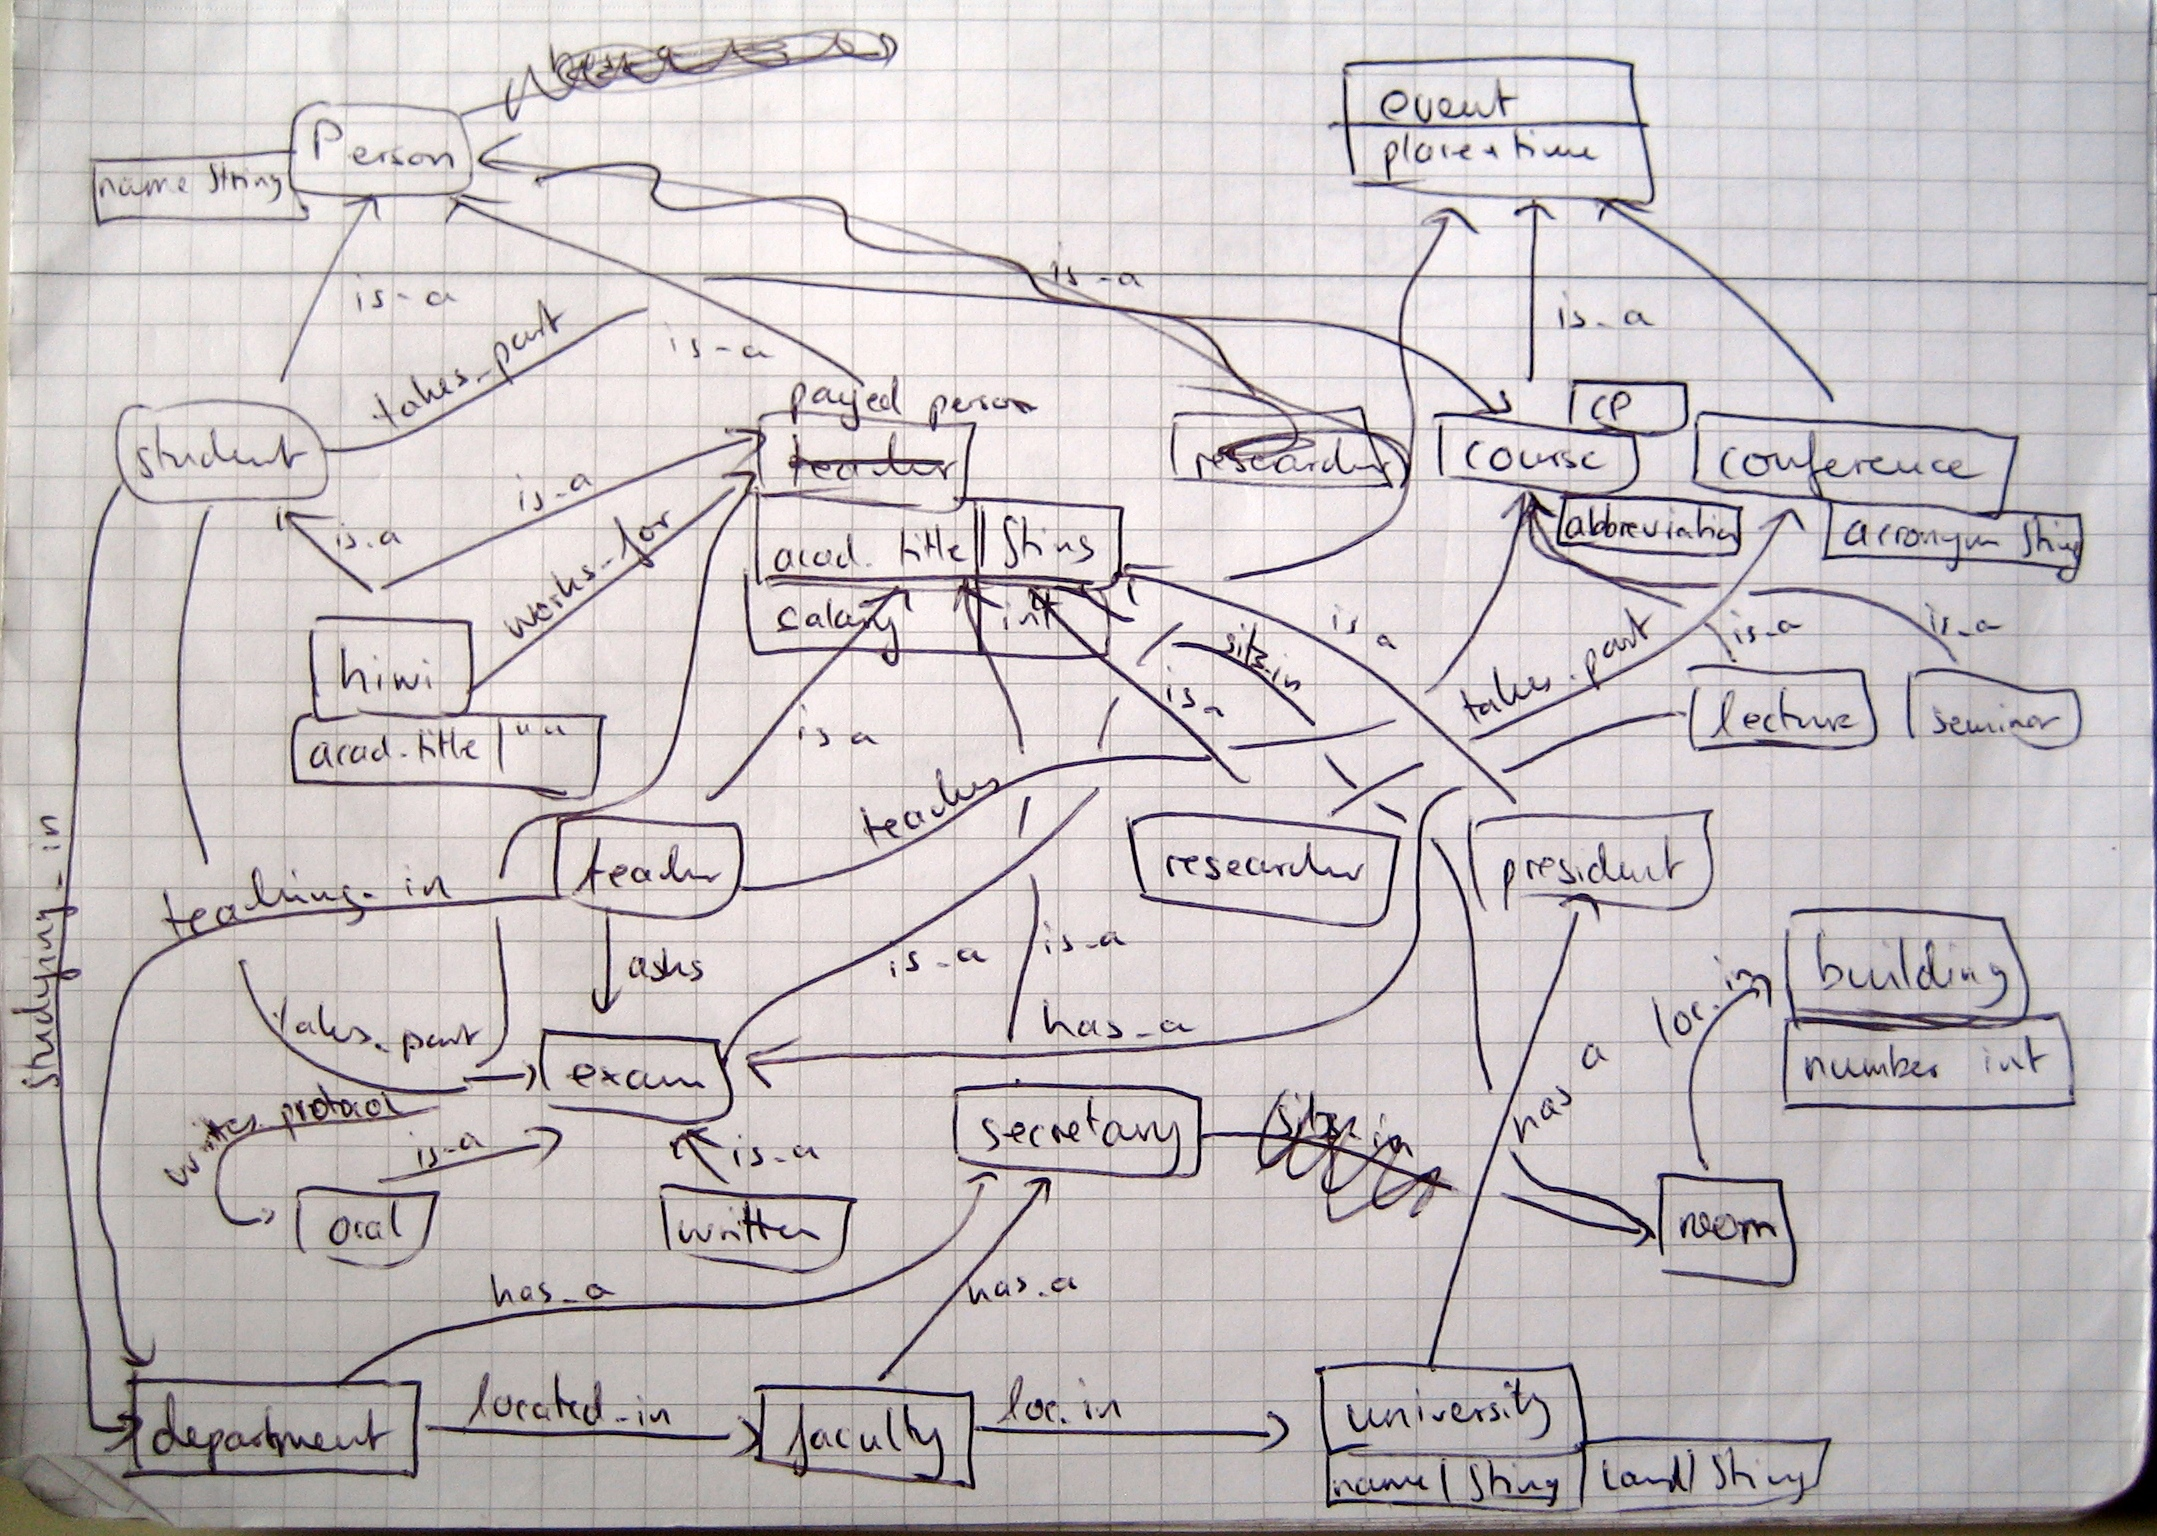
\includegraphics[width=0.25\paperwidth]{onto_1b}Nils Reiter, Graphical representations, 18.06.2006 via Flickr, Creative Commons Attribution-NonCommercial-ShareAlike\\
}
\end{frame}

\fbckg{blank} % A blank background can be used instead of an image
\begin{frame}
\sources{ % An environment for giving credit for slide backgrounds, images will need to be scaled down if there are more than two
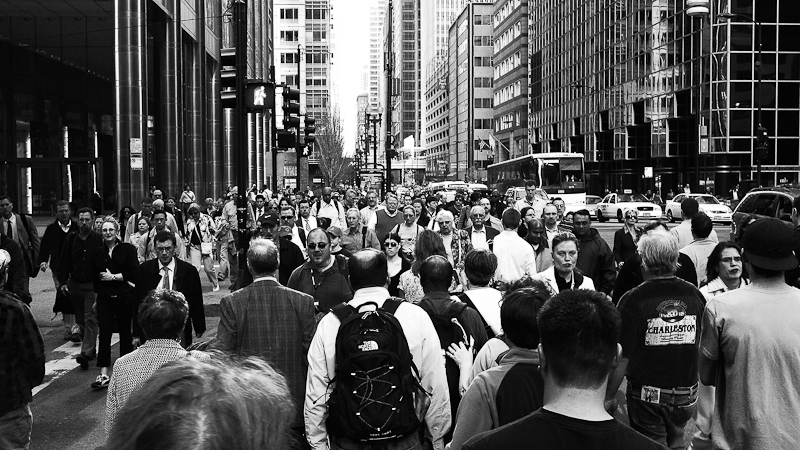
\includegraphics[width=0.25\paperwidth]{people_1}Jonathan Parker, Another Face In The Crowd, 14.04.2009 via Flickr, Creative Commons Attribution-NonCommercial-NoDerivs\\
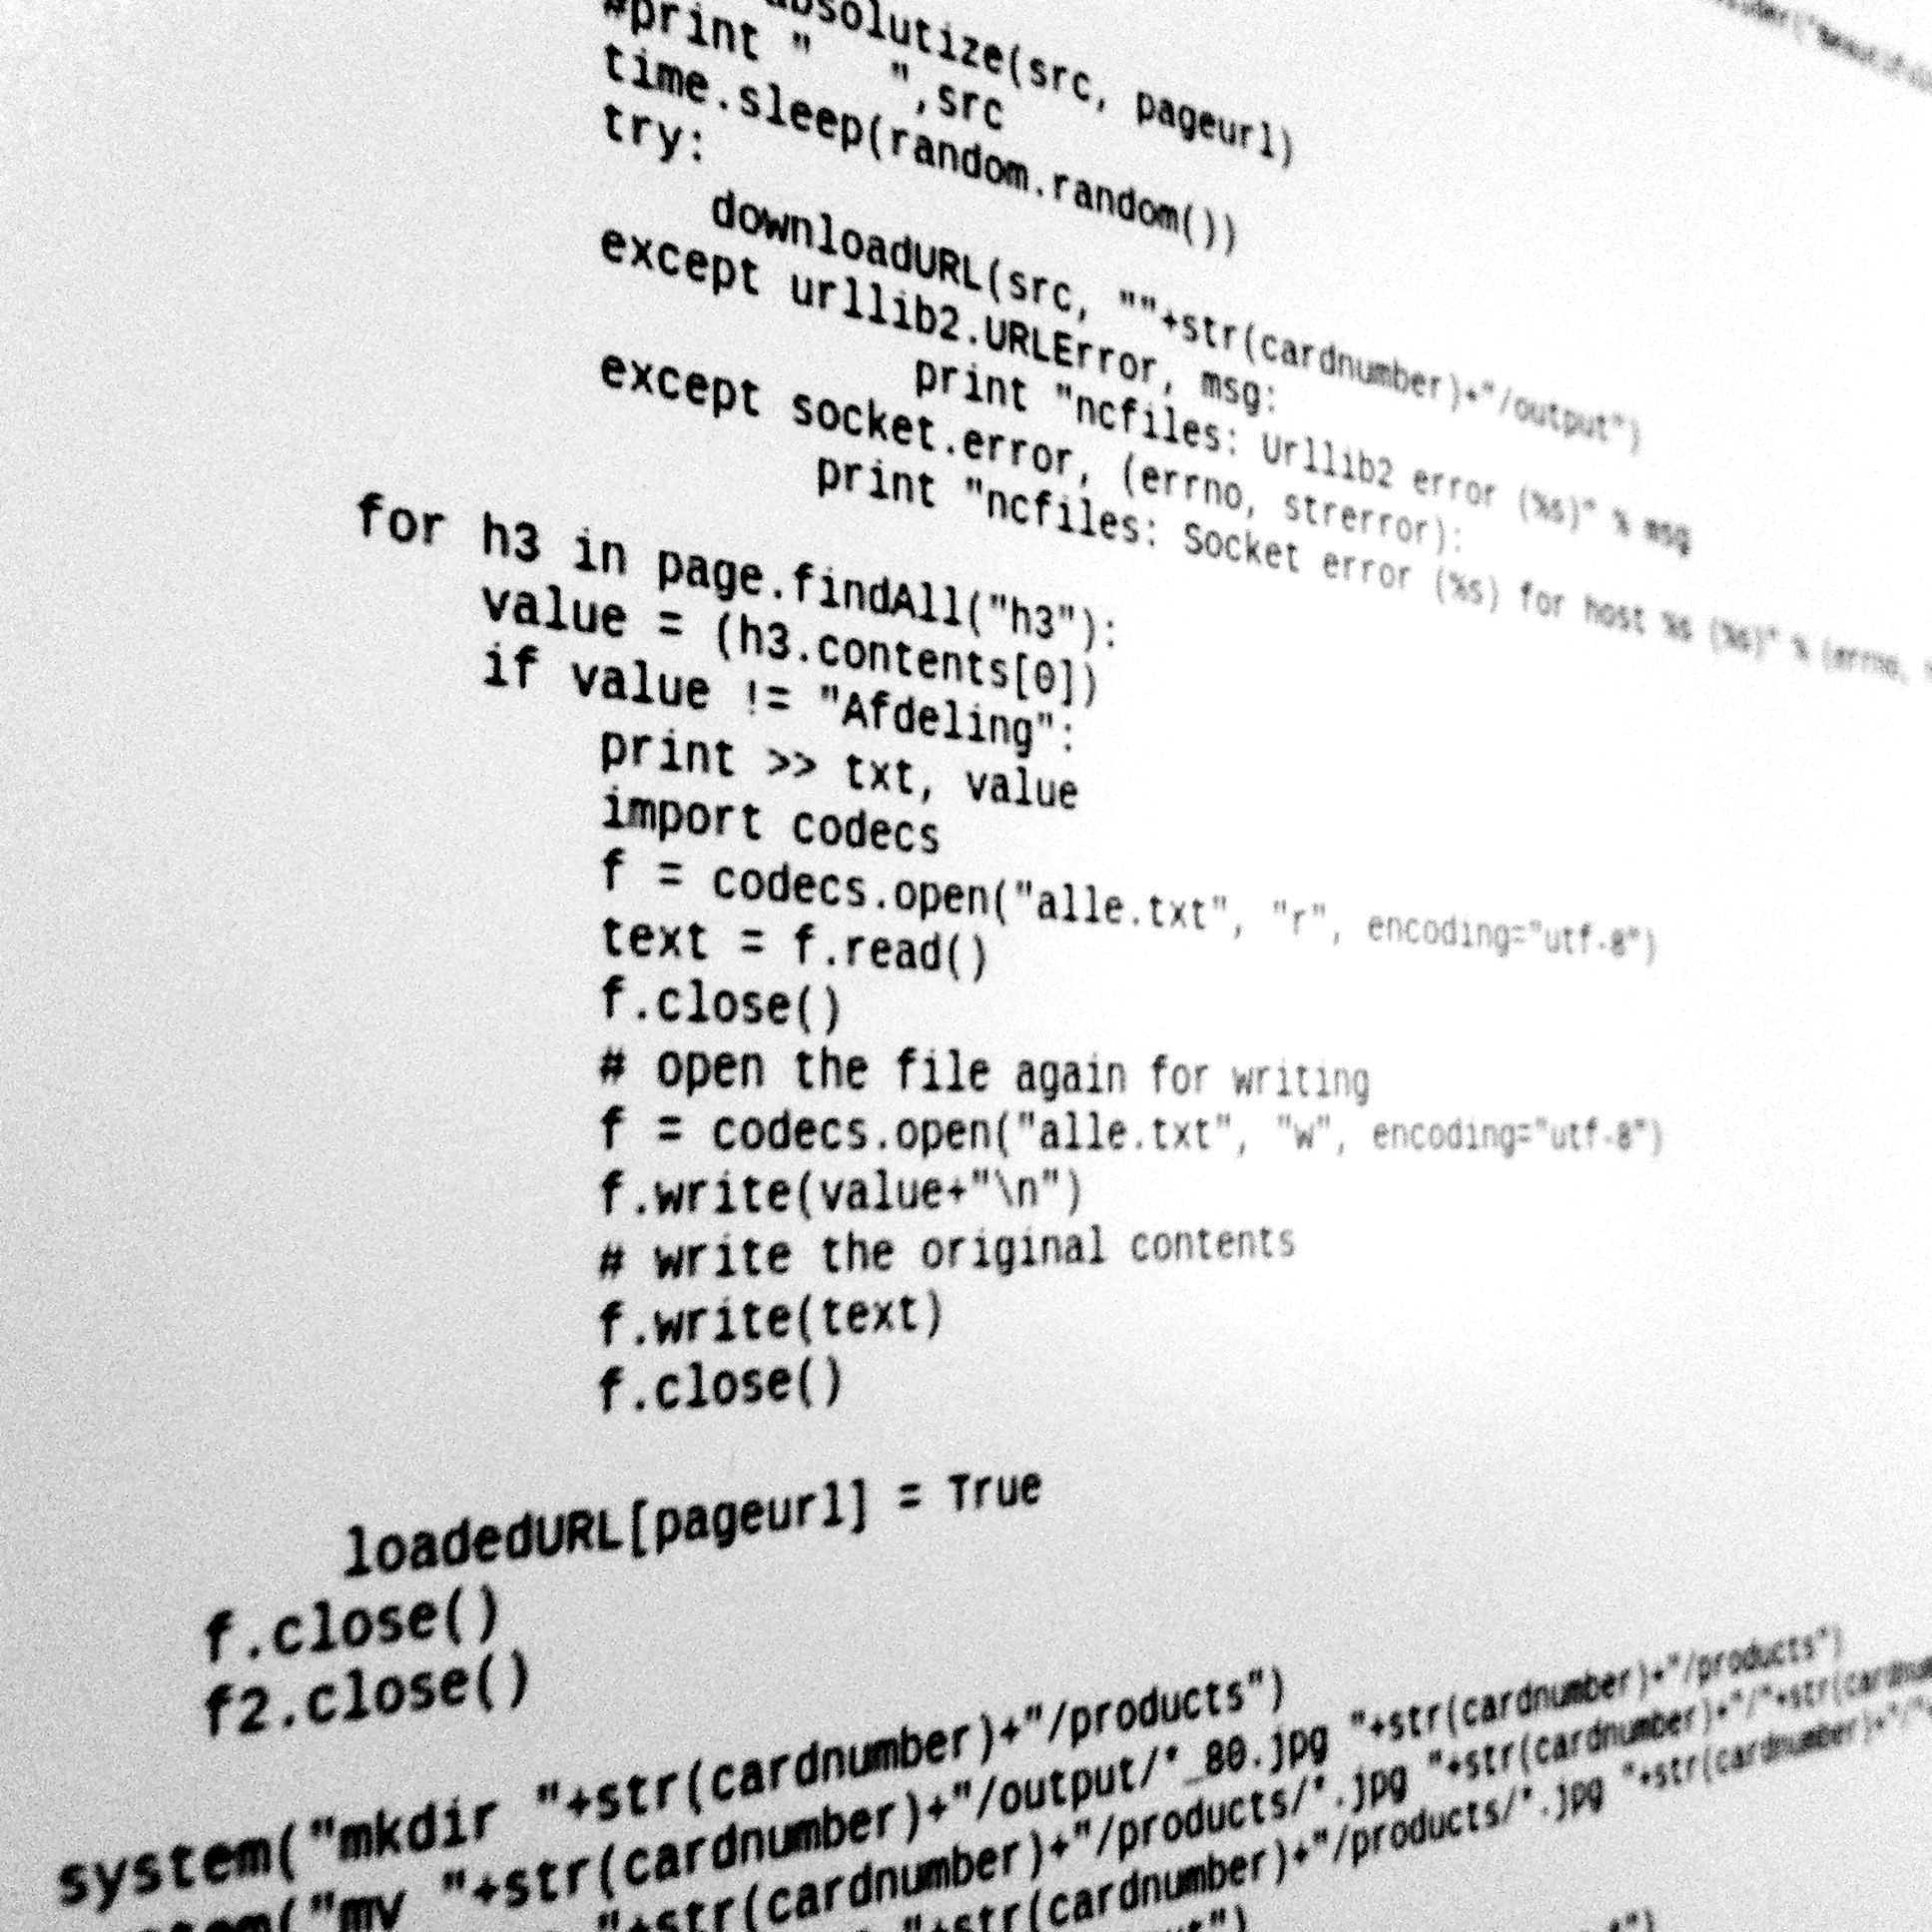
\includegraphics[width=0.25\paperwidth]{source_1}Tim Lucas, Source code ON PAPER, 22.09.2011 via Flickr, Creative Commons Attribution\\
}
\end{frame}

%----------------------------------------------------------------------------------------

\end{document}